% DO NOT COMPILE THIS FILE DIRECTLY!
% This is included by the other .tex files.
\begin{frame}[fragile]
  \frametitle{Overview}
  \begin{itemize}
    \item Upcoming computers
    \item ECP project
    \item exanauts
    \item complex networks
    \item ACOPF (Ipopt and linear solvers)
    \item SCOPF (PIPS and linear solvers)
    \item HiOp (Current-Voltage Rectangular Formulation)
    \item SIMD
    \item 


  \end{itemize}
  \begin{lstlisting}
# some julia code
println( "Here we go with Julia!")
\end{lstlisting}
\end{frame}
\begin{frame}
  \frametitle{Upcoming Supercomputers}
  \begin{columns}[T]
    \begin{column}{0.49\textwidth}
      \begin{center}
        {\bf Aurora}\\
        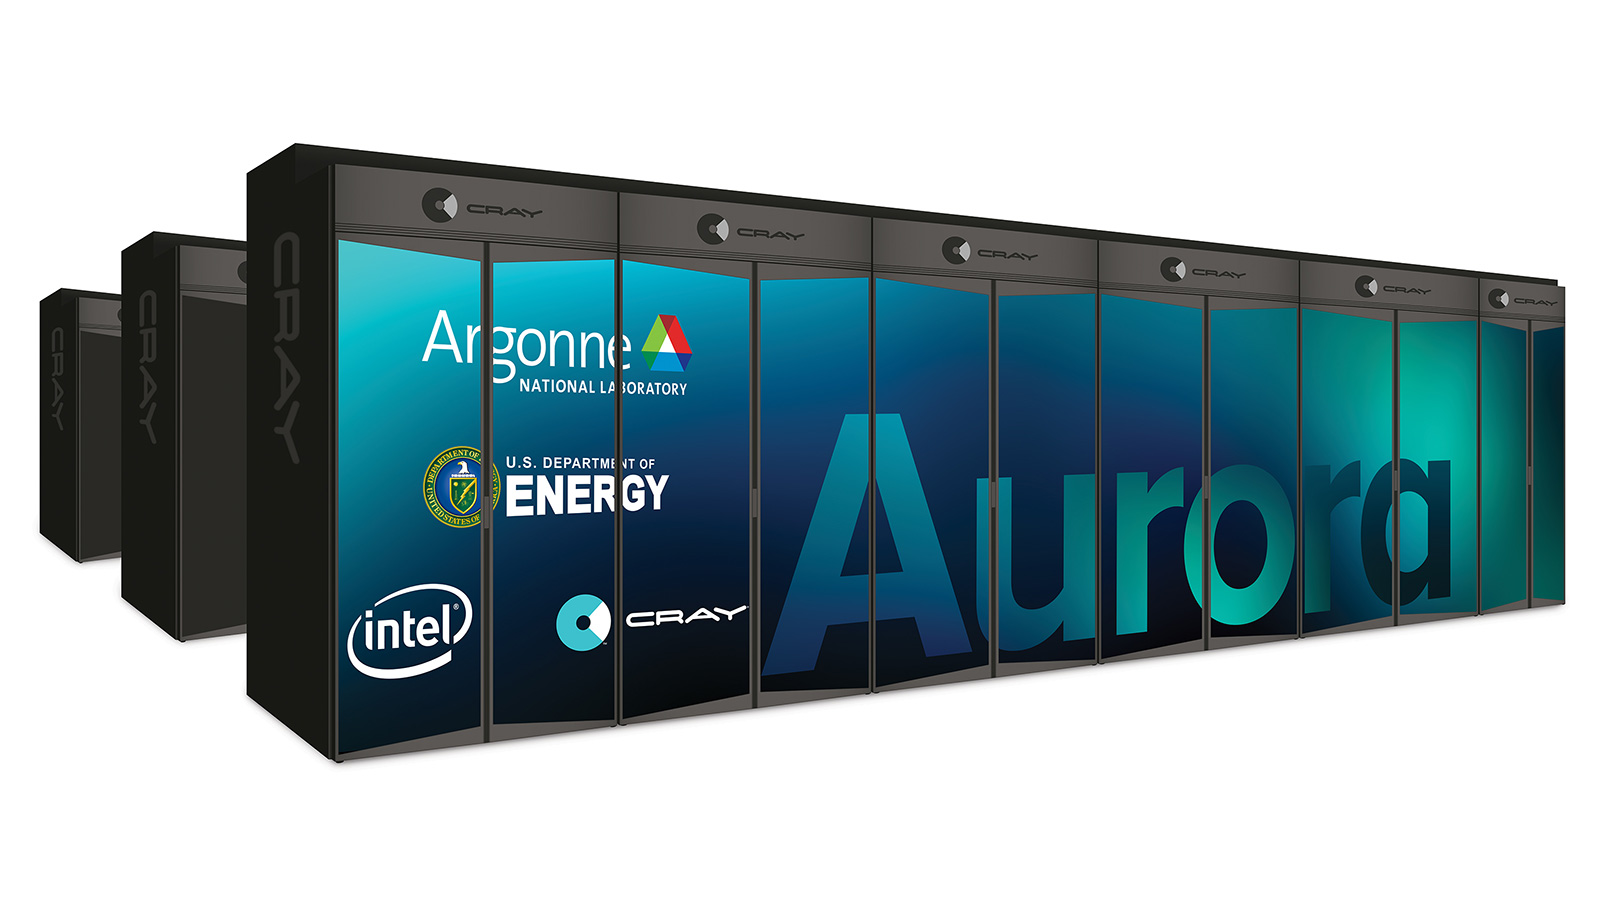
\includegraphics[width=0.75\textwidth]{./figures/aurora}
      \end{center}
    \begin{itemize}
      \item Built by Intel, subcontractor Cray
      \item $>$ 1 exaflops
      \item Built on a generation of Intel Xeon Scalable processor accelerated by Intel’s Xe compute architecture.
    \end{itemize}
    \end{column}
    \begin{column}{0.49\textwidth}
      \begin{center}
        {\bf Frontier}\\
        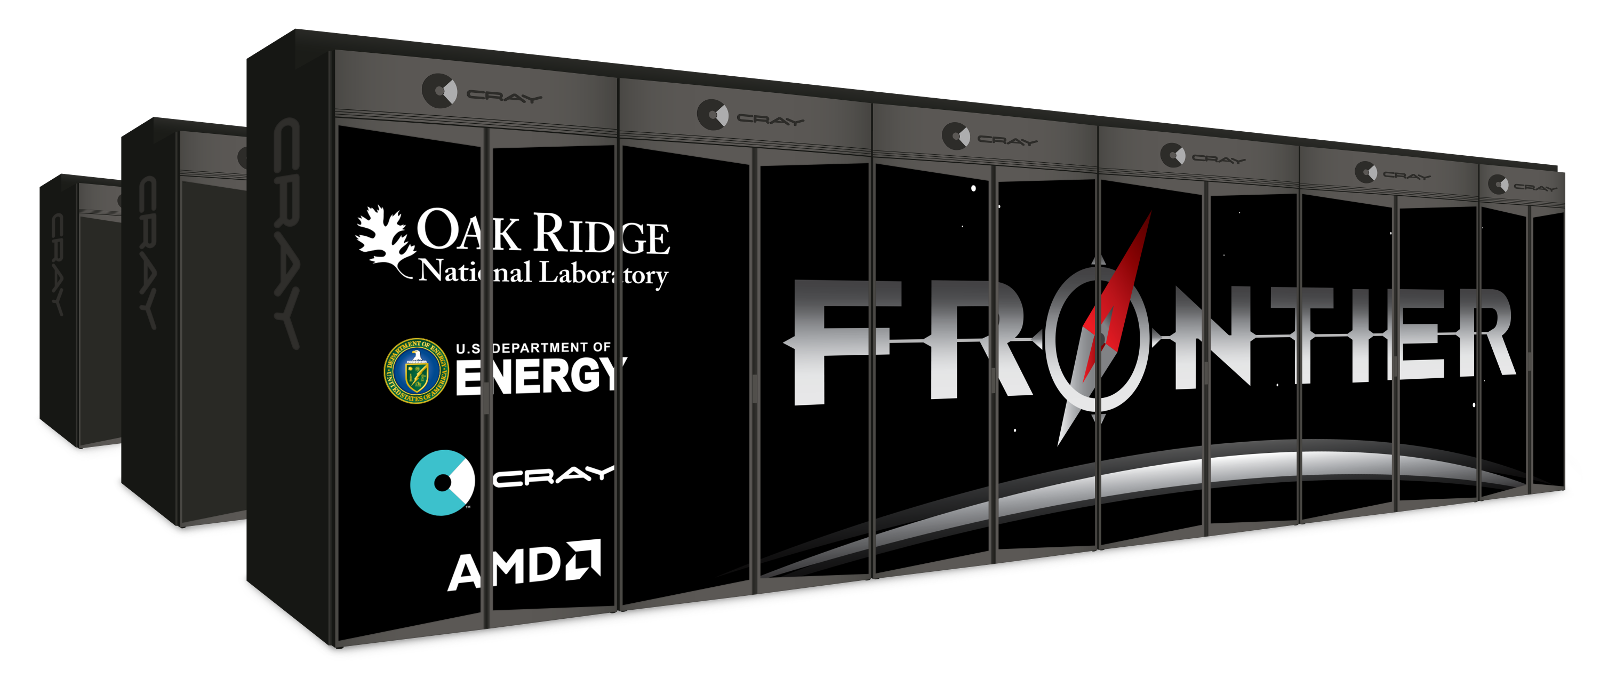
\includegraphics[width=0.75\textwidth]{./figures/frontier}
      \end{center}
      \begin{itemize}
        \item AMD EPYC processors and Radeon Instinct GPU
        \item 1.5 exaflops
        \item 2021
      \end{itemize}
    \end{column}
  \end{columns}
  \begin{itemize}
    \item No NVIDIA architecture, no CUDA
  \end{itemize}
\end{frame}

\begin{frame}
  \frametitle{Funding}
  \begin{columns}
  \begin{column}{0.45\textwidth}
    \begin{center}
      
\includegraphics[width=.75\textwidth]{./figures/ecp} \\
      % \includegraphics[width=.75\textwidth]{./figures/go} 
    \end{center}
  \end{column}
  \begin{column}{0.45\textwidth}
    \begin{center}
      % \includegraphics[width=.75\textwidth]{./figures/GMI_logo}\\
      
\includegraphics[width=.75\textwidth]{./figures/macser}
    \end{center}
  \end{column}
  \end{columns}
  \vspace{0.25cm}
  {\bf GMLC Initiative: Modernize the US Power Grid}
  \begin{itemize}
    \item Resilience of the power grid 
    \item Impact of renewables
    \item Application driven
    \item Micro grid
  \end{itemize}
  {\bf ECP Project: Optimizing Stochastic Grid Dynamics at Exascale} 
  \begin{itemize}
    \item Resilience of the power grid 
    \item Impact of renewables
    \item Computer driven
  \end{itemize}
\end{frame}

\begin{frame}
  \frametitle{Power System}
  \begin{columns}
    \begin{column}{0.45\textwidth}
      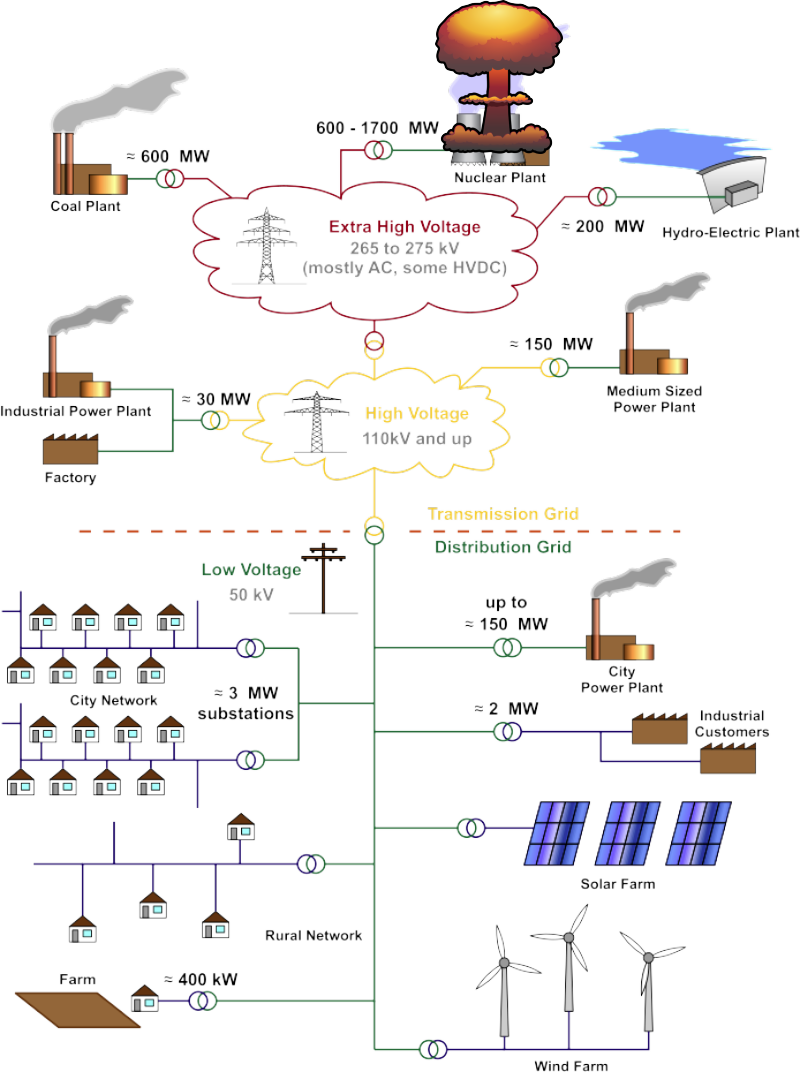
\includegraphics[width=\textwidth]{figures/slides.png}
    \end{column}
    \begin{column}{0.45\textwidth}
      \begin{center}
        % \includegraphics[width=0.8\textwidth]{figures/DampedSine.png}
      \end{center}
      \begin{itemize}
        \item Protect against contingency
        \item Demand is unknown
        \item Generation is unkown (solar, wind, water)
        \item Grid is inherently damped
        \item Steady state, power system dynamics
        \item Reduce outliers, interested in the tails
      \end{itemize}
    \end{column}
  \end{columns}
\end{frame}

\begin{frame}
  \frametitle{ExaSGD: Optimizing Stochastic Grid Dynamics at Exascale
}
\begin{columns}
  \begin{column}{0.45\textwidth}
    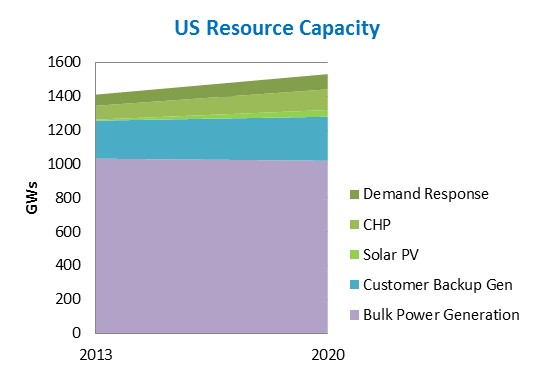
\includegraphics[width=\textwidth]{./figures/generation}
  \end{column}
  \begin{column}{0.45\textwidth}
    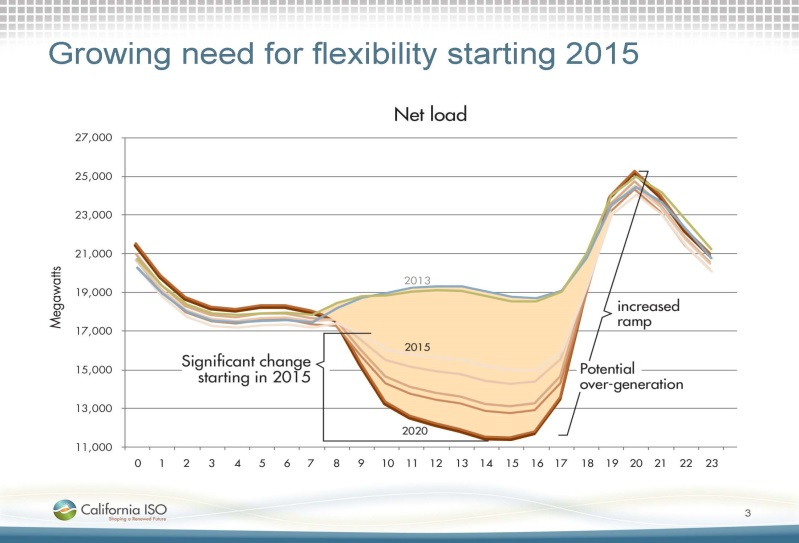
\includegraphics[width=\textwidth]{./figures/ramping}
  \end{column}
\end{columns}
  \begin{center}
      \end{center}
  {\bf Motivation:}
  \begin{itemize}
    \item More renewable energy, more uncertainty
    \item Increase in renewable energy generation ramping
  \end{itemize}
  {\bf Goals:}
  \begin{itemize}
    \item Useful long-term planning model under higher uncertainty
    \item Use AC power flow (nonlinear functions) 
    \item Efficiently leverage exascale hardware in 2021
  \end{itemize}
\end{frame}

\begin{frame}
  \frametitle{Complex Networks}
\end{frame}

\begin{frame}[fragile]
  \frametitle{Optimal Power Flow}
  \begin{itemize}
    \item {\bf Objective}
    \begin{itemize}
      \item Generation cost at generators:
      $ \minimize \sum^G_{i=1} c_i(Pg_i)$
    \end{itemize}
    \item {\bf Constraints}
    \begin{itemize}
      \item Kirchhoff's law: What flows in must flow out (nonlinear, non-convex in ACOPF)
      \begin{align*}
        V_k e^{-j\theta_k} & \sum^{N}_{m=0} (G_{km} + jB_{km})V_m e^{j\theta_m} = P - jQ,\ k = 1, \dots, N \\
        \text{where}\\
        V_k &\text{ voltage magnitude at node } k\\
        \theta &\text{ voltage angle at node } k\\
        G_{km} + jB_{km}& \text{ element of nodal admittance matrix}\\
        P, Q &\text{ net real and reactive power entering and leaving node } k
      \end{align*}
      \item Line limits \\
      $$ \theta^{min}_{nm} \leq \theta_n - \theta_m \leq \theta^{max}_{nm}$$
    \end{itemize}
  \end{itemize}
\end{frame}

\begin{frame}[fragile]
  \frametitle{Use Interior-Point for NLP}
  {\bf Solve}
  \begin{align*}
  &\minimize \phi_\mu := f(x)\\ 
  \text{with}&\\
  &g(x) \geq 0, \ i=1,\dots, m \\
  &c(x) = 0, \ j=1,\dots, l \\
  \end{align*}
  {\bf using Newton and barrier functions}
  \begin{align*}
  &\minimize \phi_\mu := f(x) - \mu \sum^m_{i=1} \ln g(x)\\ 
  \text{with}&\\
  &c(x) = 0, \ j=1,\dots, l 
  \end{align*}
  \begin{itemize}
    \item Barrier functions exacerbate ill-conditioning
  \end{itemize}
\end{frame}

\begin{frame}
      \begin{align*}
        V_k e^{-j\theta_k} & \sum^{N}_{m=0} (G_{km} + jB_{km})V_m e^{j\theta_m} = P - jQ,\ k = 1, \dots, N \\
        \text{where}\\
        V_k &\text{ voltage magnitude at node } k\\
        \theta &\text{ voltage angle at node } k\\
        G_{km} + jB_{km}& \text{ element of nodal admittance matrix}\\
        P, Q &\text{ net real and reactive power entering and leaving node } k
      \end{align*}
\end{frame}


\begin{frame}[fragile]
  \frametitle{\sout{Optimal} Power Flow}
  \begin{itemize}
    \item {\bf \sout{Objective}}
    \begin{itemize}
      \item \sout{Generation cost at generators:
      $ \minimize \sum^G_{i=1} c_i(Pg_i)$}
    \end{itemize}
    \item {\bf Constraints}
    \begin{itemize}
      \item Kirchhoff's law: What flows in must flow out (nonlinear, non-convex in ACOPF)
      \begin{align*}
        V_k e^{-j\theta_k} & \sum^{N}_{m=0} (G_{km} + jB_{km})V_m e^{j\theta_m} = P - jQ,\ k = 1, \dots, N \\
        \text{where}\\
        V_k &\text{ voltage magnitude at node } k\\
        \theta &\text{ voltage angle at node } k\\
        G_{km} + jB_{km}& \text{ element of nodal admittance matrix}\\
        P, Q &\text{ net real and reactive power entering and leaving node } k
      \end{align*}
      \item \sout{Line limits}\\
      \sout{$ \theta^{min}_{nm} \leq \theta_n - \theta_m \leq \theta^{max}_{nm}$}
    \end{itemize}
  \end{itemize}
\end{frame}

\begin{frame}[fragile]
  \frametitle{Power Flow}
  {\bf Nonlinear equations}
  \begin{itemize}
      \item Kirchhoff's law: What flows in must flow out (nonlinear, non-convex in ACOPF)
      \begin{align*}
        V_k e^{-j\theta_k} & \sum^{N}_{m=0} (G_{km} + jB_{km})V_m e^{j\theta_m} = P - jQ,\ k = 1, \dots, N \\
        \text{where}\\
        V_k &\text{ voltage magnitude at node } k\\
        \theta &\text{ voltage angle at node } k\\
        G_{km} + jB_{km}& \text{ element of nodal admittance matrix}\\
        P, Q &\text{ net real and reactive power entering and leaving node } k
      \end{align*}
      \item Use Newton-Raphson to solve nonlinear equations
  \end{itemize}
\end{frame}


\begin{frame}[fragile]
  \frametitle{BiCGSTAB}
  \begin{lstlisting}[language=julia, style=jlcodestyle]
function bicgstab(A, b, P, xi, to = nothing; tol = 1e-6, maxiter = size(A,1),
                 verbose=false)
  ...
  go = true
  iter = 1
  while go
    rhoi1 = dot(br0, ri) ; beta = (rhoi1/rhoi) * (alpha / omegai)
    pi1 .= ri .+ beta .* (pi .- omegai .* vi)
    y .= P * pi1
    vi1 .= A * y
    alpha = rhoi1 / dot(br0, vi1)
    s .= ri .- (alpha * vi1)
    z .= P * s
    t .= A * z
    t1 .= P * t
    t2 .= P * s
    omegai1 = dot(t1, t2) / dot(t1, t1)
    xi1 .= xi .+ alpha .* y .+ omegai1 .* z
  
    anorm = norm((A * xi1) .- b)
    ...

  end
  return xi, iter
end
  \end{lstlisting}
\end{frame}


\begin{frame}
  \frametitle{Multiperiod CCACOPF}
  \begin{center}
    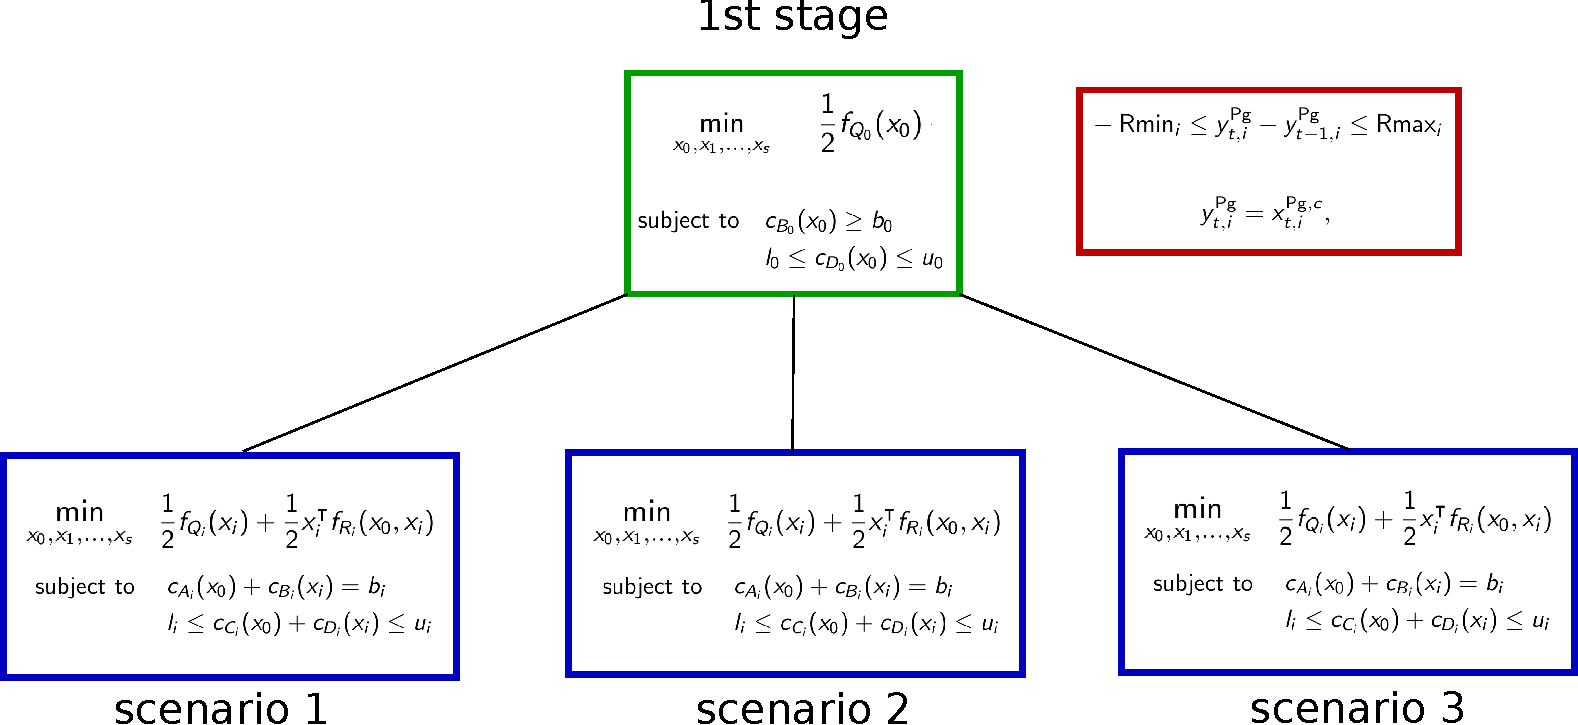
\includegraphics[width=\textwidth]{figures/twostageopt}
  \end{center}
  \begin{center}
  {\bf 1354 Bus network with 8 periods and 8192 scenarios}
    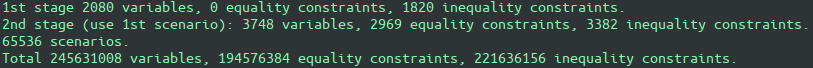
\includegraphics[width=\textwidth]{figures/generators}
  \end{center}
\end{frame}

\begin{frame}
  \frametitle{}
   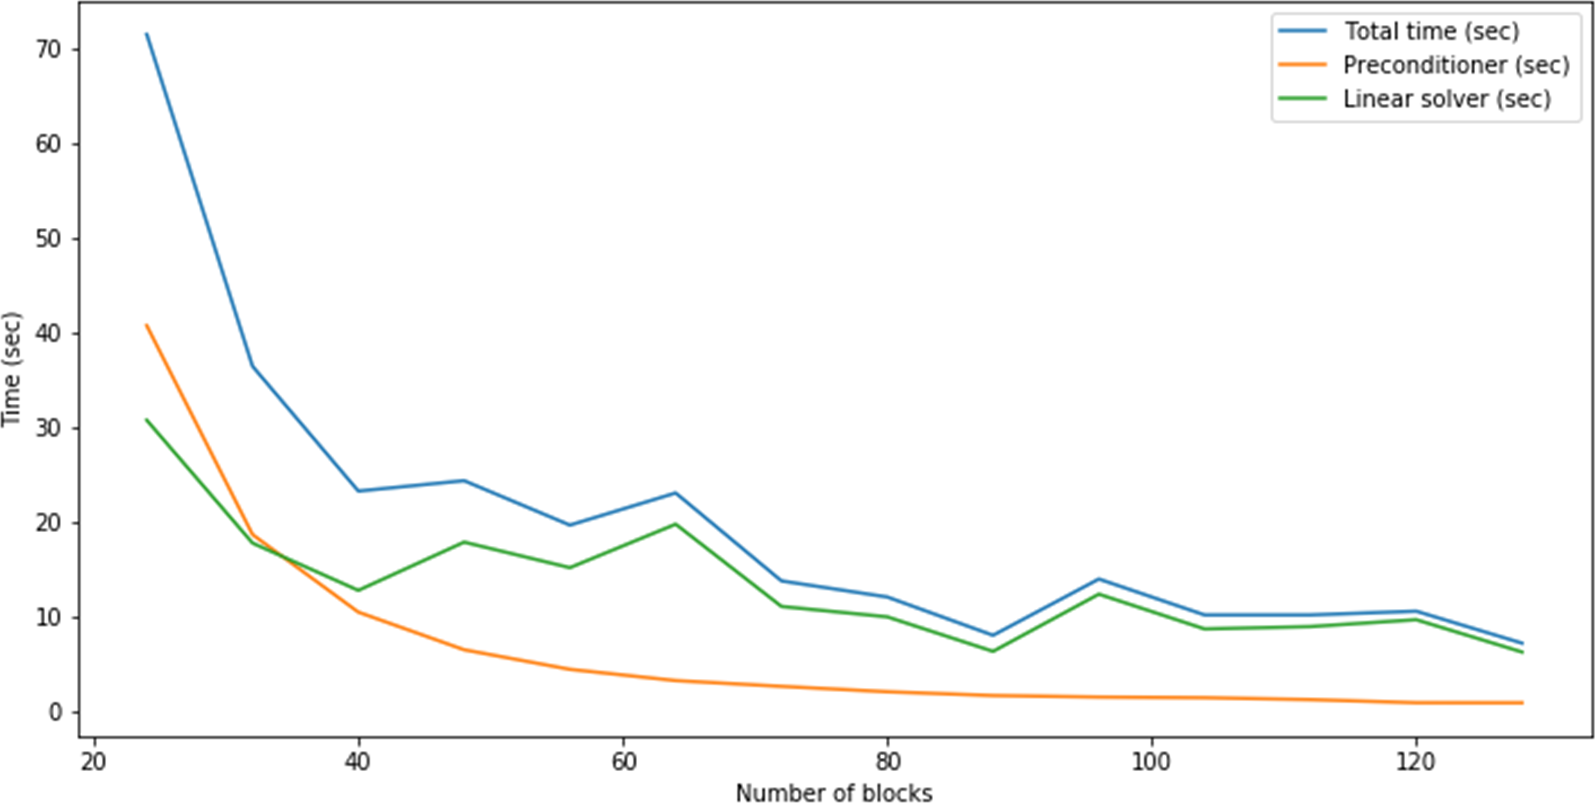
\includegraphics[width=\textwidth]{figures/blocks}
\end{frame}


\begin{frame}
  \frametitle{Two-Stage Optimization: PIPS}
  {\bf Two-Stage Problem}
\begin{equation}
  \begin{aligned}
    &\min\limits_{x_0,x_1,\dots,x_s} & & \frac{1}{2} f_{Q_0}(x_0) + 
    \frac{1}{S} \sum^{S}_{i=1} \frac{1}{2} f_{Q_i}(x_i) +  
    \frac{1}{2}x_i^{\intercal} f_{R_i}(x_0,x_i) \\
    &\mbox{subject to} & & c_{B_0}(x_0)\geq b_0 \\
    && & l_0 \leq c_{D_0}(x_0) \leq u_0 \\
    && & c_{A_i}(x_0) +c_{B_i}(x_i) = b_i \\
    && & l_i \leq c_{C_i}(x_0) + c_{D_i}(x_i) \leq u_i
  \end{aligned}
  \label{eq:opt}
  \nonumber
\end{equation}
    {\bf Linear system for Newton step inside the interior point method}
  \begin{columns}
    \begin{column}{0.3\textwidth}
  \begin{equation} 
    \left[ 
    \begin{array}{ccccc}
      K_1 & & & & B^{\intercal}_1 \\
      & K_2 & & & B^{\intercal}_2 \\
      & & \ddots & & \vdots \\
      & & & K_S & B^{\intercal}_S \\
      B_1 & B_2 & \cdots &B_S & K_0 \\
    \end{array} 
    \right] 
    \label{eq:linsys}
    \nonumber
  \end{equation} 
\end{column}
    \begin{column}{0.55\textwidth}
\[ 
\begin{array}{c}
K_i=
\left[ \begin{array}{cccc}
  \bar{Q}_i & 0 & B^{\intercal}_i & D^{\intercal}_i\\ 
  0 & D_i^s & 0 & -I \\
  B_i & 0 & D^y_i & 0 \\ 
  D_i & -I & 0 & D^z_i \\ 
\end{array} \right],\,
B_i=
\left[ \begin{array}{cccc}
  R^{\intercal}_i & 0 & A^{\intercal}_i & C^{\intercal}_i\\ 
  0 & 0 & 0 & 0 \\
  0 & 0 & 0 & 0 \\
  0 & 0 & 0 & 0 \\
\end{array} \right],
\\
K_0=
\left[ \begin{array}{cccc}
  \bar{Q}_0 & 0 & B^{\intercal}_0 &
  D^{\intercal}_0 \\ 
  0 & D_0^s & 0 & -I \\
  B_0 & 0 & D^y_0 & 0 \\ 
  D_0 & -I & 0 & D^z_0   
\end{array} \right].
\\
\end{array}
\]
\end{column}
\end{columns}
\end{frame}

\begin{frame}
  \frametitle{Why Julia?}
  \begin{center}
    
\includegraphics[width=0.2\textwidth]{./figures/julia}
  \end{center}
  \begin{itemize}
    \item User-friendly, syntax is similar to Matlab
    \item C-like performance.
    \item LLVM is supported on any upcoming supercomputer
    \item More easily (transparent) target accelerators\ldots
    \item Just-In-Time compilation allows for augmented code (automatic
      differentiation, uncertainy quantification, \ldots), not only input,
      outputs, map functions
    \item Compilation becomes part of the computation (distributed)
  \end{itemize}
\end{frame}

\begin{frame}
  \frametitle{Wishlist}
  \begin{itemize}
    \item Closer with supercomputer vendors
    \item Native optimization solver in Julia (Interior-point, active set, BFGS)
    \item Fast higher-order AD (second and third-order)
    \item Support by Cray for Julia LLVMs
    \item Support for accelerators (GPUs, FPGAs)
    \item Julia distributed parallelism based on MPI
    \item More stable APIs
  \end{itemize}
\end{frame}

\begin{frame}
  \frametitle{References}
  \footnotesize
  {\bf Links}\\
  \begin{tabular}{l}
  \href{http://julialang.org/}{http://julialang.org/} \\
  \href{https://github.com/StructJuMP/StructJuMP.jl}{https://github.com/StructJuMP/StructJuMP.jl}
  \\
  \href{https://github.com/Argonne-National-Laboratory/PIPS}{https://github.com/Argonne-National-Laboratory/PIPS}\\
  \href{https://gitlab.com/michel2323/multi-period-ac-opf}{https://gitlab.com/michel2323/multi-period-ac-opf}\\
  \end{tabular}


  {\bf ExaSGD}
  \begin{center}
    \begin{tabular}{ccc}
      {\bf PNNL} & {\bf ANL} & {\bf NREL} \\
      Zhenyu (Henry) Huang & Mihai Anitescu & Wesley Jones \\
      Bruce Palmer & Emil Constantinescu & Bri-Mathias Hodge \\
      Jesse Holzer&  Francois Gilbert & Matthew Reynolds\\
      Poorva Sharma & Kibaek Kim & Devon Sigler \\
      Yuri Makarov &  Cosmin Petra  (LLNL)  & Ryan King\\
      Stephen Elbert  &Adrian Maldonado& Clayton Barrows \\
      Shriang Abhankar &  Michel Schanen \\
      Gary Black \\
    \end{tabular}
  \end{center}
  {\bf PIPS-NLP}
  \begin{center}
    \begin{tabular}{ccc}
      Cosmin Petra & Victor Zavala & Naiyuan Chiang \\
    \end{tabular}
  \end{center}
  {\bf StructJuMP}\\
  \begin{center}
    \begin{tabular}{ccc}
      Cosmin Petra (LLNL) & Feng Qiang (ANL) & Joey Huchette (MIT)\\
      Miles Lubin (MIT)\\
    \end{tabular}
  \end{center}
\end{frame}




